% Basic schematic describing the structure of the app.
% \documentclass[transparent]{standalone}
\documentclass[crop,tikz,convert={outext=.svg,command=\unexpanded{pdf2svg \infile\space\outfile}},multi=false]{standalone}[2012/04/13]

% \usepackage{tikz}
\usetikzlibrary{shapes.geometric, arrows}

\tikzset{every picture/.style={/utils/exec={\sffamily}}}

\begin{document}

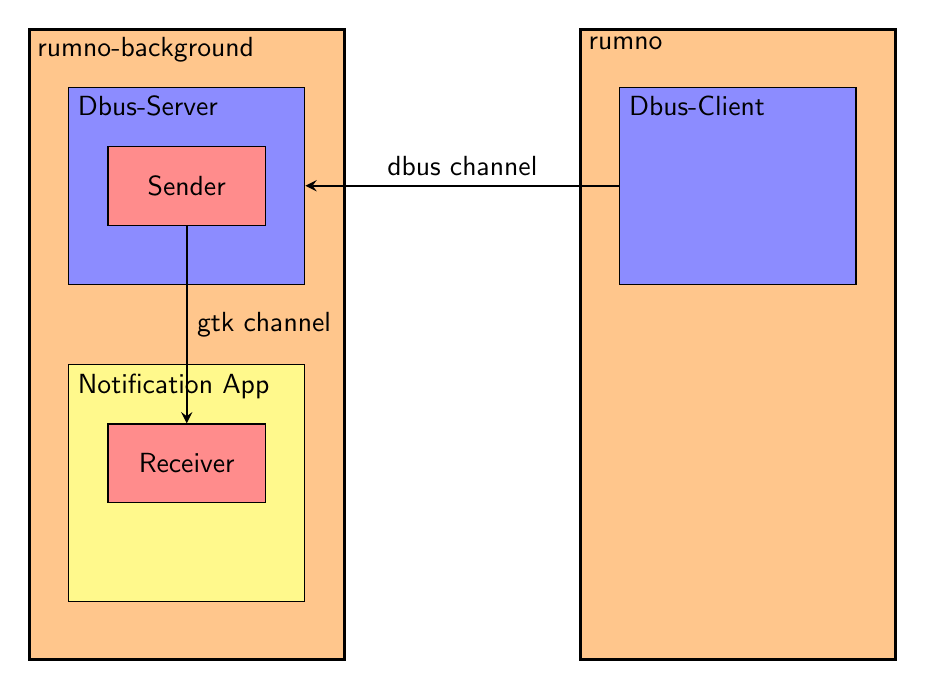
\begin{tikzpicture}
    % Define some common parameters
    \def\margin{0.75cm}
    \def\distanceMain{6cm}
    \def\colorSaturation{45}

    % Define styles
    \tikzstyle{E1} = [rectangle, minimum width=4cm, minimum height=8cm, line width=0.4mm, draw=black, fill=orange!\colorSaturation]
    \tikzstyle{E2} = [rectangle, minimum width=3cm, minimum height=2.5cm, draw=black, fill=blue!\colorSaturation]
    \tikzstyle{E3} = [rectangle, minimum width=3cm, minimum height=3cm, draw=black, fill=yellow!\colorSaturation]
    \tikzstyle{E4} = [rectangle, minimum width=2cm, minimum height=1cm, text centered, draw=black, fill=red!\colorSaturation]

    \tikzstyle{arrow} = [thick,->,>=stealth]

    % Finaly draw everything
    \node (server) [E1] at (0,0) {};
    \node[below right] at (server.north west) {rumno-background};
    \node[below] at (server.north) (dbus_server) [E2, yshift=-\margin] {};
    \node[below right] at (dbus_server.north west) {Dbus-Server};
    \node[above] at (dbus_server.south) (sender) [E4, yshift=\margin] {Sender};

    \node[above] at (server.south) (notification_app) [E3, yshift=\margin] {};
    \node[below right] at (notification_app.north west) {Notification App};
    \node[below] at (notification_app.north) (receiver) [E4, yshift=-\margin] {Receiver};


    \node (client) [E1, right of=server, xshift=\distanceMain] {};
    \node[below right] at (client.north west) {rumno};
    \node[below] at (client.north) (dbus_client) [E2, yshift=-\margin] {};
    \node[below right] at (dbus_client.north west) {Dbus-Client};

    \draw [arrow] (dbus_client) -- node[anchor=south] {dbus channel} (dbus_server);

    \draw [arrow] (sender) -- node[anchor=west] {gtk channel} (receiver);

\end{tikzpicture}


\end{document}
